\documentclass[tikz,border=0pt]{standalone}
\usepackage{fontspec}
\setmainfont{TeX Gyre Heros}
\setsansfont{TeX Gyre Heros}
\usepackage{amssymb}
\usetikzlibrary{arrows.meta,positioning}
% Shared visual language for Cosmon diagrams. Included after tikz is loaded.
\ifdefined\lightmode
  \definecolor{CosmonBg}{HTML}{E8EFE7}
  \definecolor{CosmonInk}{HTML}{172019}
  \definecolor{CosmonMuted}{HTML}{59665B}
  \definecolor{CosmonFaint}{HTML}{AAB7AA}
  \definecolor{CosmonPanel}{HTML}{F4F7F2}
  \definecolor{CosmonAccent}{HTML}{176D2B}
\else
  \definecolor{CosmonBg}{HTML}{08090C}
  \definecolor{CosmonInk}{HTML}{E7E9E7}
  \definecolor{CosmonMuted}{HTML}{969D97}
  \definecolor{CosmonFaint}{HTML}{444A45}
  \definecolor{CosmonPanel}{HTML}{101317}
  \definecolor{CosmonAccent}{HTML}{3FB950}
\fi

\colorlet{CosmonRoadmap}{CosmonMuted}

\tikzset{
  cosmon text/.style={font=\sffamily\color{CosmonInk}},
  cosmon micro/.style={font=\sffamily\fontsize{6.4}{7.7}\selectfont, text=CosmonMuted},
  cosmon small/.style={font=\sffamily\fontsize{7.4}{9}\selectfont, text=CosmonInk},
  cosmon label/.style={font=\sffamily\bfseries\fontsize{7.2}{8.6}\selectfont, text=CosmonMuted},
  cosmon title/.style={font=\sffamily\bfseries\fontsize{11}{13}\selectfont, text=CosmonInk},
  cosmon frame/.style={draw=CosmonFaint, line width=.55pt, rounded corners=4pt},
  cosmon panel/.style={draw=CosmonFaint, fill=CosmonPanel, line width=.45pt, rounded corners=3pt},
  cosmon molecule/.style={circle, fill=CosmonInk, minimum size=3.6pt, inner sep=0pt},
  cosmon dependency/.style={draw=CosmonMuted, line width=.5pt, -{Latex[length=2.5pt,width=2.1pt]}},
  cosmon data/.style={draw=CosmonInk, line width=1.6pt, {Latex[length=3.1pt,width=2.5pt]}-{Latex[length=3.1pt,width=2.5pt]}},
  cosmon outbound/.style={draw=CosmonAccent, line width=1.05pt, -{Latex[length=3.4pt,width=2.8pt]}},
  cosmon exchange/.style={draw=CosmonInk, line width=.75pt, {Latex[length=3pt,width=2.4pt]}-{Latex[length=3pt,width=2.4pt]}},
  cosmon roadmap/.style={draw=CosmonRoadmap, line width=.65pt, dashed, dash pattern=on 2.4pt off 2.2pt},
  cosmon roadmap arrow/.style={cosmon roadmap, {Latex[length=2.7pt,width=2.2pt]}-{Latex[length=2.7pt,width=2.2pt]}},
  cosmon slot/.style={draw=CosmonAccent, line width=1.2pt, rounded corners=.7pt},
  cosmon peer/.style={circle, draw=CosmonRoadmap, dashed, line width=.6pt, minimum size=13pt, inner sep=0pt},
}

% Canonical glyphs: use these in both diagrams and in the generated legend.
\newcommand{\PilotGlyph}{\textcolor{CosmonAccent}{\ensuremath{\blacklozenge}}}
\newcommand{\MoleculeGlyph}{\textcolor{CosmonInk}{\ensuremath{\bullet}}}
\newcommand{\TraceGlyph}{\textcolor{CosmonAccent}{\ensuremath{\therefore}}}

% The detailed figure's one and only legend, built from the same styles as the art.
\newcommand{\CosmonLegend}{%
  \begin{scope}[shift={(0,0)}]
    \draw[cosmon dependency] (.60,.30) -- (1.22,.30);
    \node[cosmon micro, anchor=west] at (1.36,.30) {thin = ordering dependency};
    \draw[cosmon data] (4.38,.30) -- (5.00,.30);
    \node[cosmon micro, anchor=west] at (5.14,.30) {thick = content in shared files};
    \draw[cosmon roadmap] (8.83,.30) -- (9.45,.30);
    \node[cosmon micro, anchor=west] at (9.59,.30) {dashed = roadmap};
    \node[cosmon micro, anchor=west] at (11.82,.30)
      {\PilotGlyph\ pilot\quad \MoleculeGlyph\ molecule\quad \TraceGlyph\ durable trace};
  \end{scope}%
}


\begin{document}
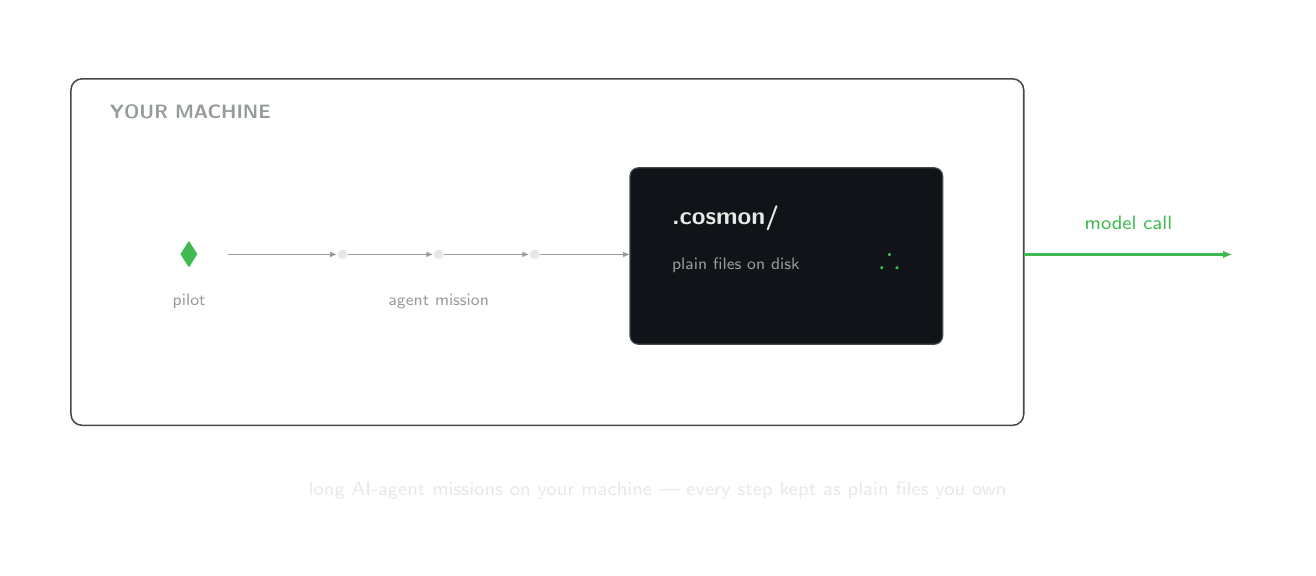
\begin{tikzpicture}[x=1cm,y=1cm]
  \useasboundingbox (0,0) rectangle (16,6.6);

  \draw[cosmon frame] (.55,1.55) rectangle (12.65,5.95);
  \node[cosmon label, anchor=west] at (.92,5.53) {YOUR MACHINE};

  \node[cosmon title, anchor=center] (pilot) at (2.05,3.72) {\PilotGlyph};
  \node[cosmon micro, anchor=north] at (2.05,3.34) {pilot};

  \node[cosmon molecule] (a1) at (4.00,3.72) {};
  \node[cosmon molecule] (a2) at (5.22,3.72) {};
  \node[cosmon molecule] (a3) at (6.44,3.72) {};
  \draw[cosmon dependency] (2.55,3.72) -- (a1);
  \draw[cosmon dependency] (a1) -- (a2);
  \draw[cosmon dependency] (a2) -- (a3);
  \node[cosmon micro, anchor=north] at (5.22,3.34) {agent mission};

  \draw[cosmon panel] (7.65,2.58) rectangle (11.62,4.82);
  \node[cosmon small, font=\sffamily\bfseries\fontsize{9}{10.5}\selectfont, anchor=west]
    at (8.06,4.18) {.cosmon/};
  \node[cosmon micro, anchor=west] at (8.06,3.58) {plain files on disk};
  \node[cosmon title, anchor=east] at (11.20,3.69) {\TraceGlyph};
  \draw[cosmon dependency] (a3) -- (7.65,3.72);

  \draw[cosmon outbound] (12.65,3.72) -- (15.30,3.72);
  \node[cosmon small, text=CosmonAccent, anchor=south] at (13.98,3.91) {model call};

  \node[cosmon small, anchor=center, text width=15cm, align=center]
    at (8,.72) {long AI-agent missions on your machine --- every step kept as plain files you own};
\end{tikzpicture}
\end{document}
